

\begin{figure}[hbt]
\centering
%\includegraphics[scale=0.39]{figures/scanfigures/.pdf}
FIGURE
\caption{Cross--section (fb) per bin of $(M_{jj},\,\Delta y_{jj})$ at NLO QCD $\mathcal{O}(\alpha_{ew}^6\alpha_s)$, without any cut on the $jj$ pair kinematics. Results of \texttt{XXX} calculations.}\label{fig:mjjdyjj_2d_NLO}
\end{figure}
\newpage

% \subsection{Validity of the VBS approximation}\label{subsec:VBSapprox}

The VBS approximation [?] is frequently employed for VBS computations and we aim at the identification of kinematical regions where it provides trustworthy prediction for the $W^+W^+$ scattering.
At LO, given the full set of diagrams contributing at order $\mathcal{O}(\alpha_{ew}^6)$, the approximations consists in:
\begin{itemize}
\item discarding interferences between $t$ and $u$ channel diagrams, which are expected to be suppressed in the fiducial volume, after VBF cuts;
\item discarding $s$--channel diagrams shown in \autoref{fig:jjpeak_diag}, which contain $q\bar{q}'$ annihilations ($W^-\rightarrow q \bar{q}'$); with a hard cut on the $jj$--pair invariant mass, these contributions are strongly suppressed.
\end{itemize}

\begin{figure}[hbt]
\centering
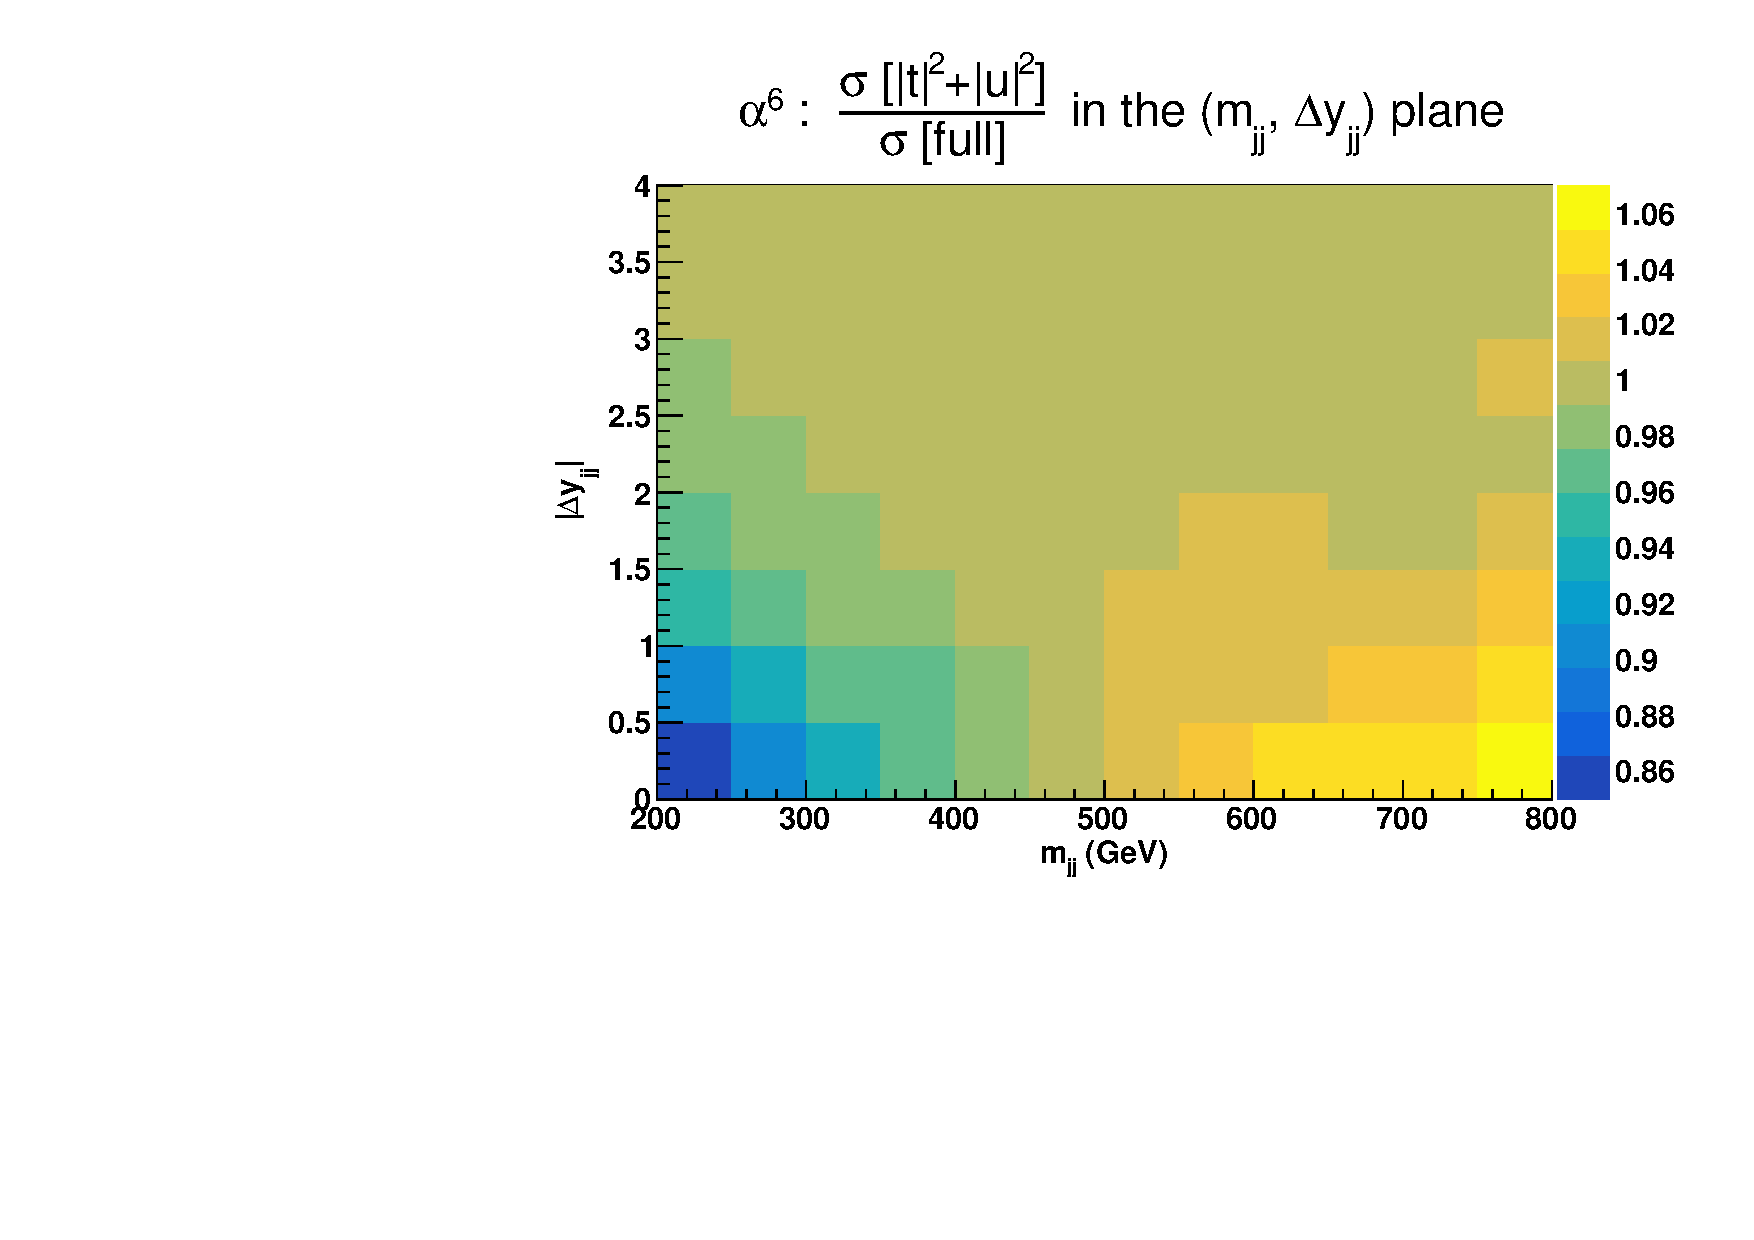
\includegraphics[scale=0.395]{figures/scanfigures/ratio_tu.pdf}
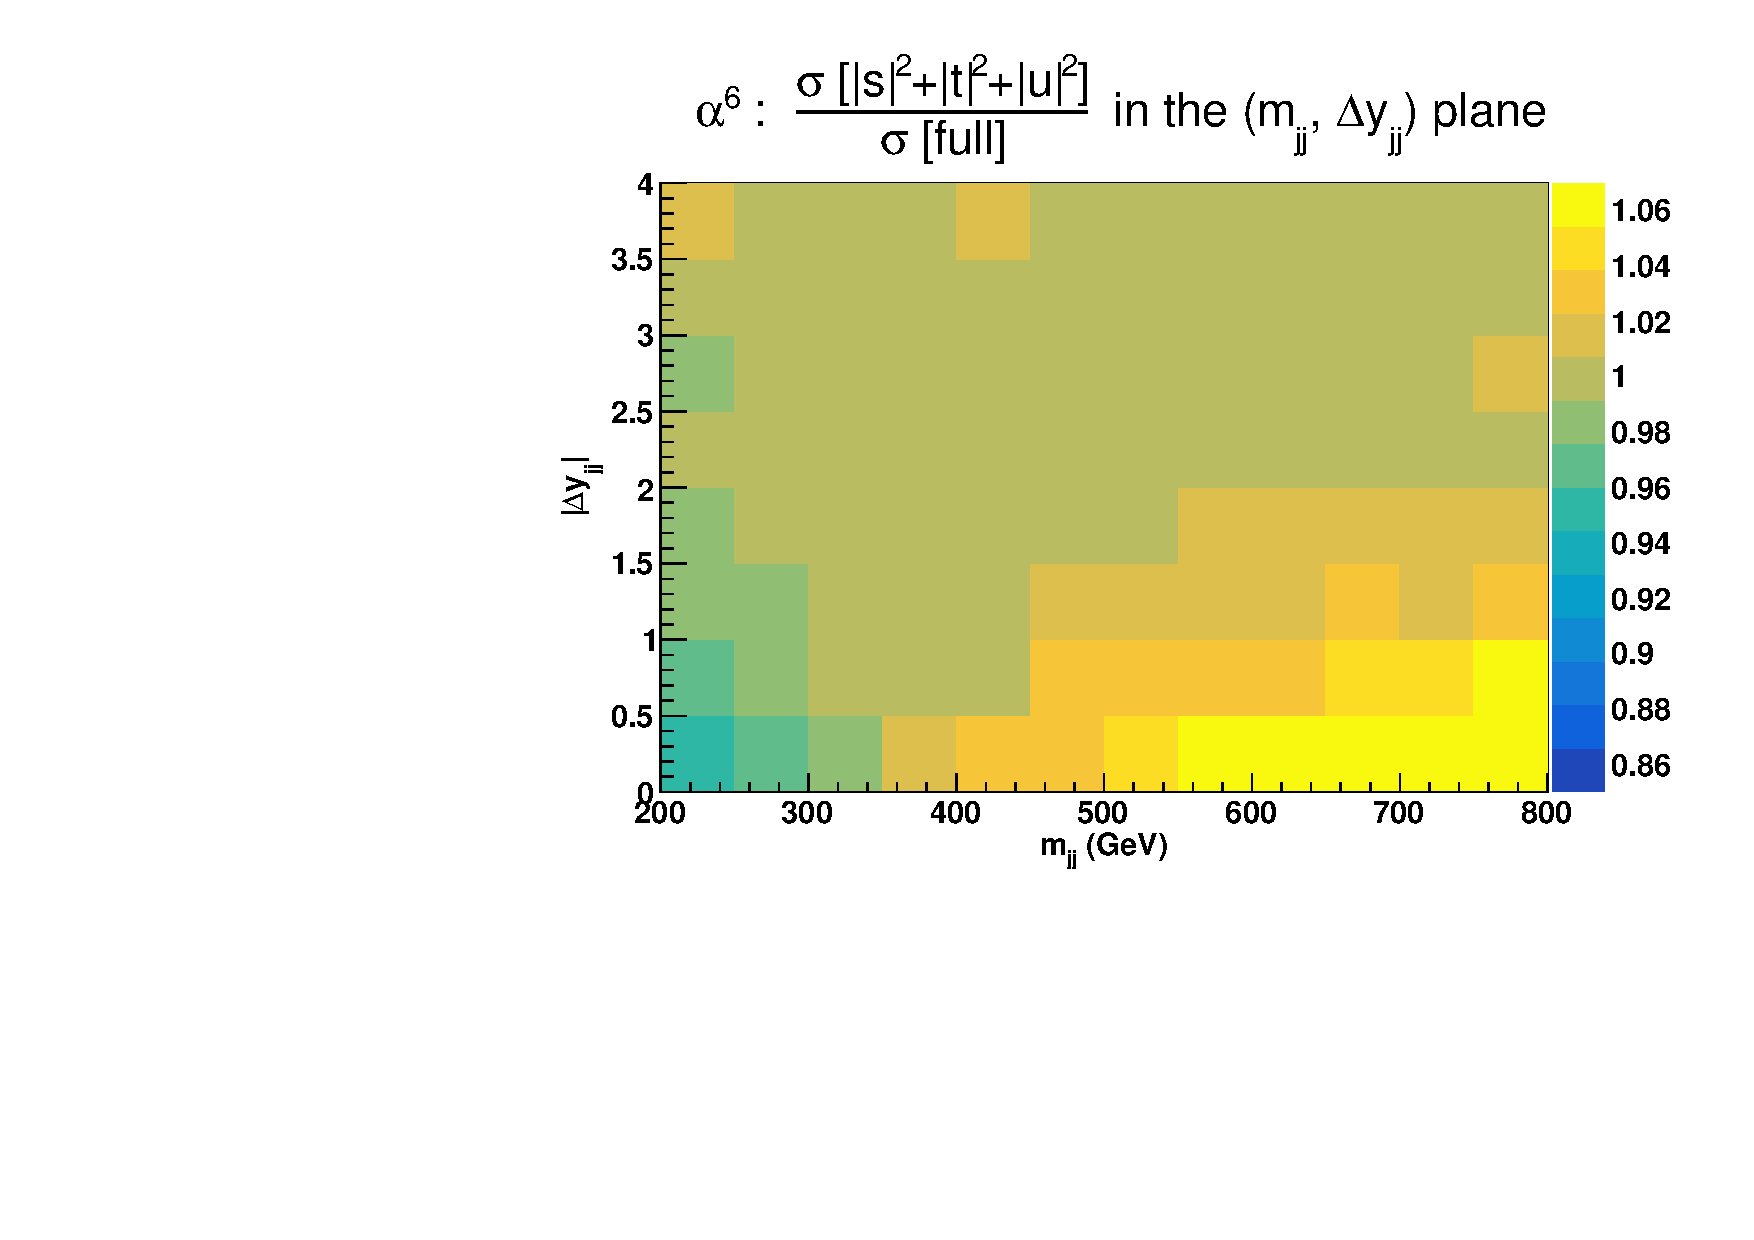
\includegraphics[scale=0.395]{figures/scanfigures/ratio_stu.pdf}
\caption{Cross--sections (fb) per bin of $(M_{jj},\,\Delta y_{jj})$ at $\mathcal{O}(\alpha_{ew}^6)$, without any cut on the $jj$ pair kinematics: ratio of approximated squared amplitudes over the full matrix element. The approximated squared amplitudes are computed as $|\mathcal{A}|^2 \sim |t|^2 + |u|^2$ (left) and $|\mathcal{A}|^2 \sim |s|^2 + |t|^2 + |u|^2$ (right). Results of \texttt{VBFNLO} (approximated) and \texttt{PHANTOM} (full) calculations.}\label{fig:ratio2d_LO}
\end{figure}

\begin{figure}[hbt]
\centering
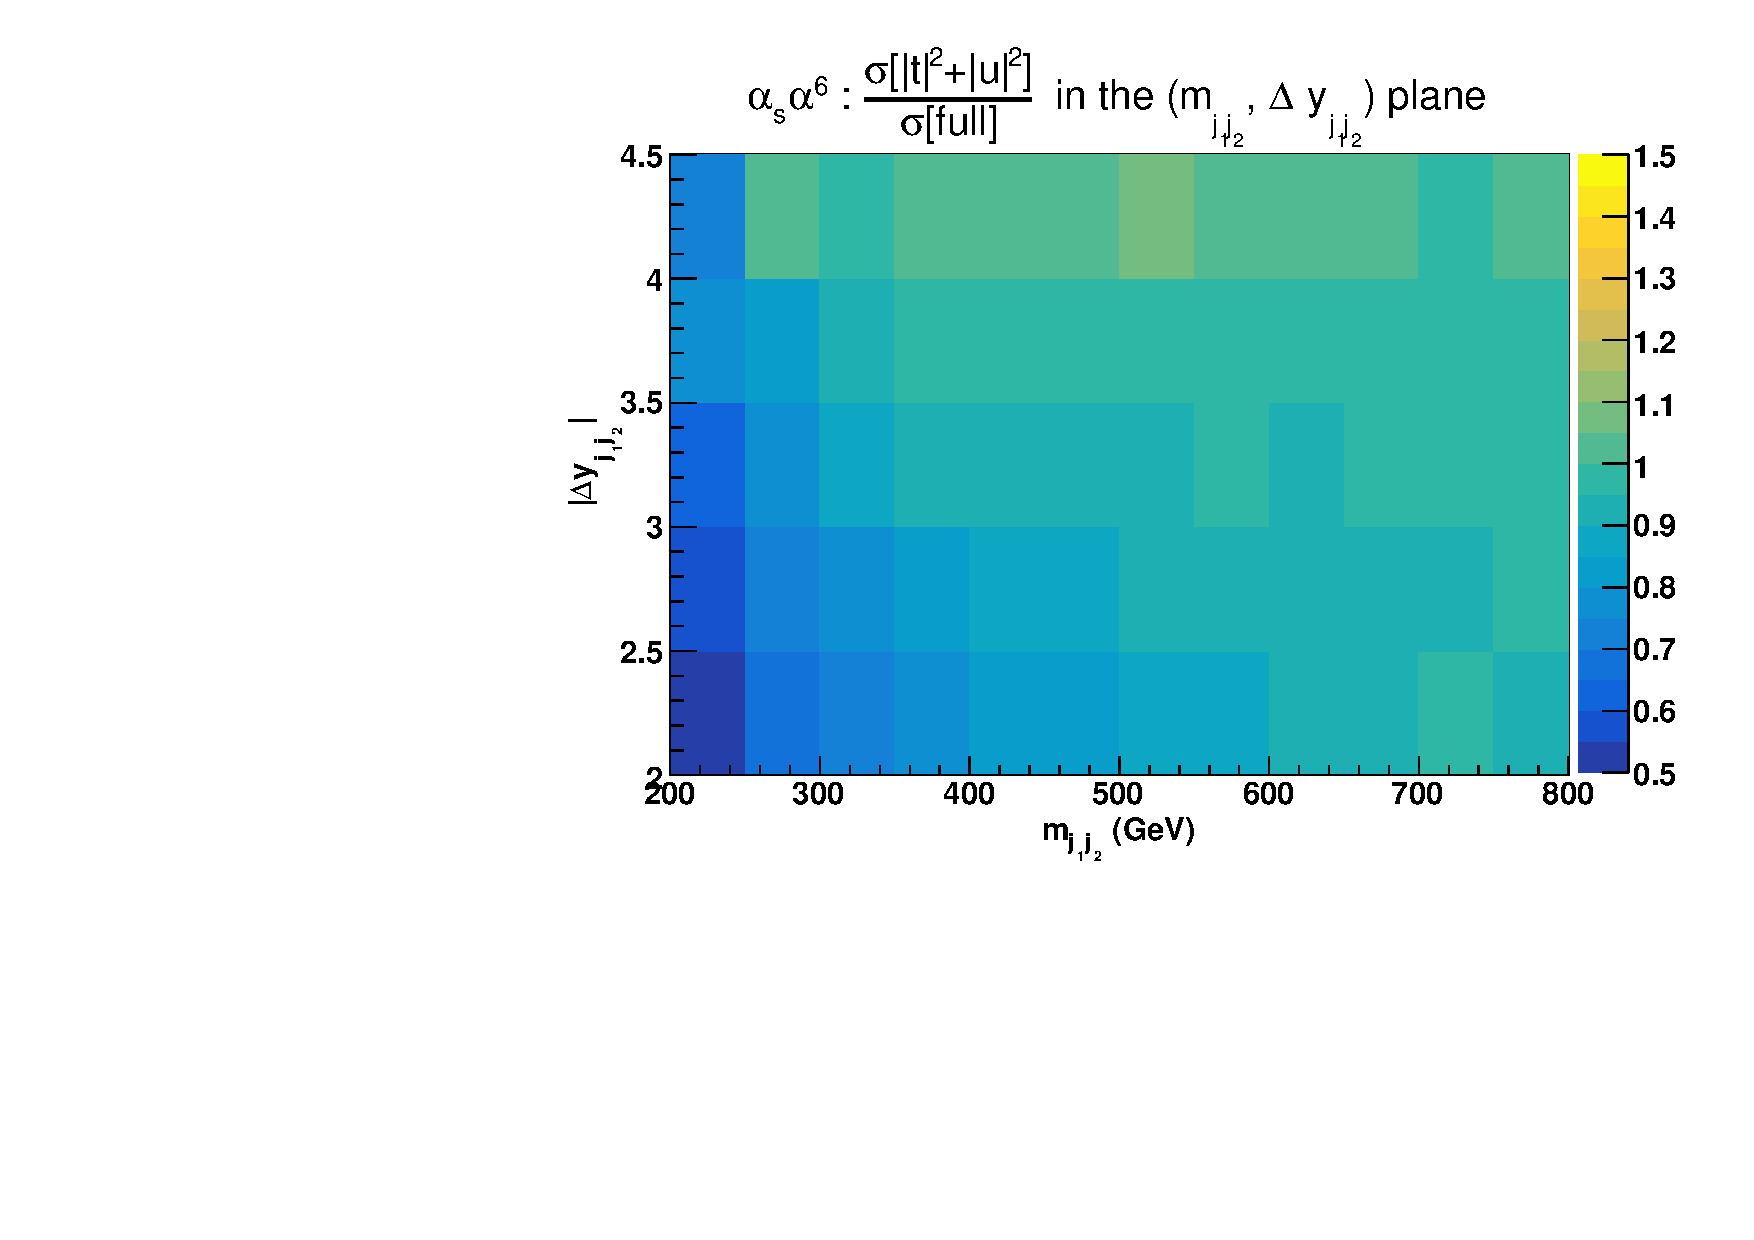
\includegraphics[scale=0.395]{figures/scanfigures/a6as_vbfnloVSrecola_tu.pdf}
%\includegraphics[scale=0.395]{figures/scanfigures/.pdf}
\caption{Cross--sections (fb) per bin of $(M_{jj},\,\Delta y_{jj})$ at $\mathcal{O}(\alpha_{ew}^6\alpha_s)$, without any cut on the $jj$ pair kinematics: ratio of approximated squared amplitudes over the full matrix element. The approximated squared amplitudes are computed as $|\mathcal{A}|^2 \sim |t|^2 + |u|^2$ (left) and $|\mathcal{A}|^2 \sim |s|^2 + |t|^2 + |u|^2$ (right). Results of \texttt{VBFNLO} (approximated) and \texttt{RECOLA} (full) calculations. RIGHT SIDE FIG. IN PREPARATION. QUESTION: is RECOLA calc. 'exact' ?}\label{fig:ratio2d_NLO}
\end{figure}